\documentclass{report}
\usepackage{tikz}
\usepackage[utf8]{inputenc}
\usepackage{graphicx}
\usepackage{fancyhdr}
\pagestyle{fancy}

\title{ISAKMP}
\author{arfritz97 }
\date{August 2019}

\newcommand{\squash}{\itemsep=0pt\parskip=0pt}

\title{Understanding ISAKMP/IKE}
\author{Anna Fritz \\
  Information and Telecommunication Technology Center \\
  The University of Kansas \\
  \url{arfritzz@ku.edu}

\begin{document}

\maketitle

\chapter {Understanding ISAKMP}

Below is an inital overview of the capabilites of ISAKMP where ISAKMP outlines framework for authentication and key exchange but is key exchange independent. Then, IKE is key dependent where the procedure for IKE occurs in two phases where phase one is when two entities agree on how to protect further negotiation traffic while negotiating an ISAKMP SA for an authenticated and secure channel. Phase two is when the secure channel is then used to negotiate security services for IPSec.

\begin{itemize}
  \squash
\item ISAKMP is the protocol for establishing Security Associations (SA) and cryptographic keys in an internet environment.
\item ISAKMP is a part of IKE.
  \begin{itemize}
     \squash
	\item IKE establishes the shared security policy and authenticated keys.
	\item ISAKMP uses IKE for key exchange.
	\end{itemize}
\item Defines payloads for exchanging key generation and authentication data.
\item Allows an entity's initial communications to indicate which certificate authorities (CAs) it supports.
\item Overall, 4 goals
  \begin{enumerate}
     \squash
	\item authenticating a communicating peer
	\item creation and management of security associations
	\item key generation techniques
	\item threat mitigation
	\end{enumerate}
\end{itemize}

Since a SA is the main goal, it is necessary to understand what a security association is. A SA is uniquely identified by three parameters (4) consisting of:
\begin{itemize}
\item Security Parameter Index (SPI) (identifies the SA)
\item IP destination address
\item Security protocol (AH or ESP) identified
\end{itemize}

\section {ISAKMP Header}

\subsection {Header Fields}

\begin{itemize}
   \squash
\item Initiator Cookie (8 octects) = Cookie of entity that initiated SA establishment, notification, or deletion.
\item Responder Cookie (8 octects) = Cookie of responder 
\item Next Payload (1 octet) = Type of first payload
\item Major/Minor Version (4 bits each) = Version of ISAKMP in use
\item Exchange Type (1 octet) = Type of exchange being used
\item Flags (1 octet) = More stinking flags, encrypt, commit authentication only
\item Message ID (4 octets) = Unique ID to identify things in Phase 2
\item Length (4 octets) = Length of total message (header + payload)
\end{itemize}

\subsection {Next Payload Types}

The following list details the possible next payload types as well as thier associated values.

\begin{itemize}
  \squash
\item NONE = 0
\item SA = 1
\item Proposal = 2
\item Transofrm = 3
\item Key Exchange = 4
\item Identification = 5
\item Certificate = 6
\item Cert Request = 7
\item Hash = 8
\item Signature = 9
\item Nonce = 10
\item Notification = 11
\item Delete = 12
\item Vendor ID = 13
\item Reserves = 14-127
\item Private Use = 128-225
\end{itemize}

\subsection {Exchange Types}

The next aspect that is necessary to define is the exchange type. This is useful as it tells the responder the desired exchange specifications such as fast exchange or slow exchange. The follow list details the exchange types with their associated values. 

\begin{itemize}
   \squash
\item NONE = 0
\item Base = 1
\item Id Protection = 2
\item Auth Only = 3
\item Aggressive = 4
\item Informational = 5
\item ISAKMP Future Use = 6 - 31
\item DOI Specific Use = 32 - 127
\item Private Use = 128 - 255
\end{itemize}

\subsection {Payload Headers}

Payload headers can be generic or customized for the situation. A generic header simply includes Payload Data where the Data can change based on the situation. 

\section {SA Payload}

The Domain of Interpretation (DOI) and Situation are included in the Security Association payload. Some details about the Domain of Interpretation and Situation can be seen below.

\begin{itemize}
\item DOI (4 octets) = Identifies the DOI under which negotiation takes place. A value of 0 during Phase 1 specifies a Generic ISAKMP SA which can be used for any protocol during Phase 2.
\item Situation = A DOI-specific field that identifies the situation under which this negotiation is taking place. 
\end{itemize}

\section {Proposal Payload}

The proposal payload carries many unique aspects as seen with the following list below

\begin{itemize}
\item Payload Length = Length is octets of the entire Proposal payload including the generic payload header, the Proposal payload, and all Transform payloads associated with this proposal.
\item Proposal Number = identifies the proposal number for the current payload
\item Proposal ID = Specifies the protocol identifier such as IPSEC ESP, IPSEC AH, OSPF, TLS, etc.
\item SPI Size = Length in octets of the SPI as defined by the Protocol ID
\item No. of Transforms = Specifies the number of transforms for the proposal.
\item SPI (variable) = sending entity's SPI
\end{itemize}

\section {Transform Payload}

The unique thing about transform payloads is they include a Transform Number and a Tranform ID. The Transform number identifies the transform number for the current payload. The Transform ID specifies the transform identifier for the protocol within the current proposal. 

\section {Key Exchange Payload}

This payload includes key exchange data which could be of variable length. It is the data required to generate a session key and is specified by the DOI and the associated Key Exchange algorithm.

\section {Certificate Payload}

This payload includes cert encoding which indicates the type of certified contained in the certificate field. 

\section{Final Outcome}

Once the Security Association (SA) has been established, the following will be agreed upon by both the initiator and the responder:

\begin{itemize}
\item Encryption algorithm
\item ISAKMP hash algorithm
\item Diffie-Hellman modulus
\item SA lifetime
\item Authentication parameters (RSA signatures, RSA nonces, pre-shared keys)
\end{itemize}

With that, the following options are listed before for each of the different categories agreed upon in the SA. 

\begin{itemize}
  \squash
\item an authentication method (ensure id of peers)
  \begin{itemize}
 \squash
  \item rsa-sig = digital certificate with keys generated by RSA signature algorithm
  \item crack = challenge/response for authenticated cryptographic keys
  \item pre-share (default) = preshared keys
  \end{itemize}
\item an encryption method (protect data and ensure privacy)
  \begin{itemize}
 \squash
  \item des = 56-bit DES-CBS
  \item 3des (default) = 168-bit Triple DES
  \item aes = advanced encryption standard supports lengths 128, 192, 256 bits
  \item aes-192
  \item aes-256  
  \end{itemize}
\item Hashed Message Authentication Codes (HMAC) (ensure message has not been modified in transit)
  \begin{itemize}
 \squash
  \item sha (default) = SHA-1 (HMAC variant)
  \item md5 = MD5 (HMAC variant)
  \end{itemize}
\item a Diffie-Hellman group to determine strength of the encryption-key-determination algorithm
  \begin{itemize}
 \squash
  \item 1 = Group 1 (768-bit)
  \item 2 = Group 2 (1024-bit)
  \item 5 = Group 5 (1536-bit)
  \item 7 = Group 7 (Elliptical curve field size is 163 bits)
  \end{itemize}
\item a limit to the time the SA is valid
  \begin{itemize}
 \squash
  \item integer value (86400 is default) = 120 to 2147483647 seconds
  \end{itemize}

\chapter {Proposal Syntax}

Perhaps it is most important to understand the composition of a proposal to understand ISAKMP. Proposals with the same Proposal number are taken as a logical AND and Proposals with different numbers are taken as the logical OR. Different transform within a proposal are taken as the logical OR.

Since the communication between parties could involve one or multiple computers, each ISAKMP policy is assigned a unique priority number between 1 and 10,000 where policy 1 has the highest priority. It is common practice to start numbering at 10 in case you must insert a policy with a higher priority. (1).

\section {Parameters Necessary}

Before creating a security association, both parties, the initator and responser must agree on the following parameters:

\begin{enumerate}
  \squash
\item encryption algorithm
\item ISAKMP hash algorithm
\item what Diffie-Hellman modulus will be used
\item lifetime
  \begin{itemize}
  \item shorter SA lifetime = more secure
  \item If shorter, when one party goes down, in some cases the SA doesn't expire until its lifetime ends.
  \end{itemize}
\item Authentication Parameter (RSA signatures, RSA nonces and pre-shared keys)
  \begin{itemize}
  \item RSA Signatures = the most secure but least utilized becuase it requires deploying and managing a certificate authority server
  \item RSA Nonce = random number encrypted by recipient's public key. The downside is the communicating peer must have the public keys of all other peers which it communicates with and that enforces a great deal of labor.
    \item Pre-shared keys = least secure but commonly used to authenticate gateway peers
  \end{itemize}
\end{enumerate}


\section {Proposal Example}


The base exchange then follows these steps:

\begin{enumerate}
\squash
\item The Initiator sends the proposal to Responder to begin ISAKMP-SA negotiation
\item The Responder responds with HDR, SA, Nonce resulting in the basic SA being agreed 
\item The Initiator responds with Header, KE, IDii, and Auth which includes the key generated by the responder (KE) and the Initiator identity verified (Idii)
\item The Responder responds with HDR, KE, Idir, Auth which includes the responder ident verified (KE) and the initiator key generated (IDir). The security association (SA) is established. 
\end{enumerate}

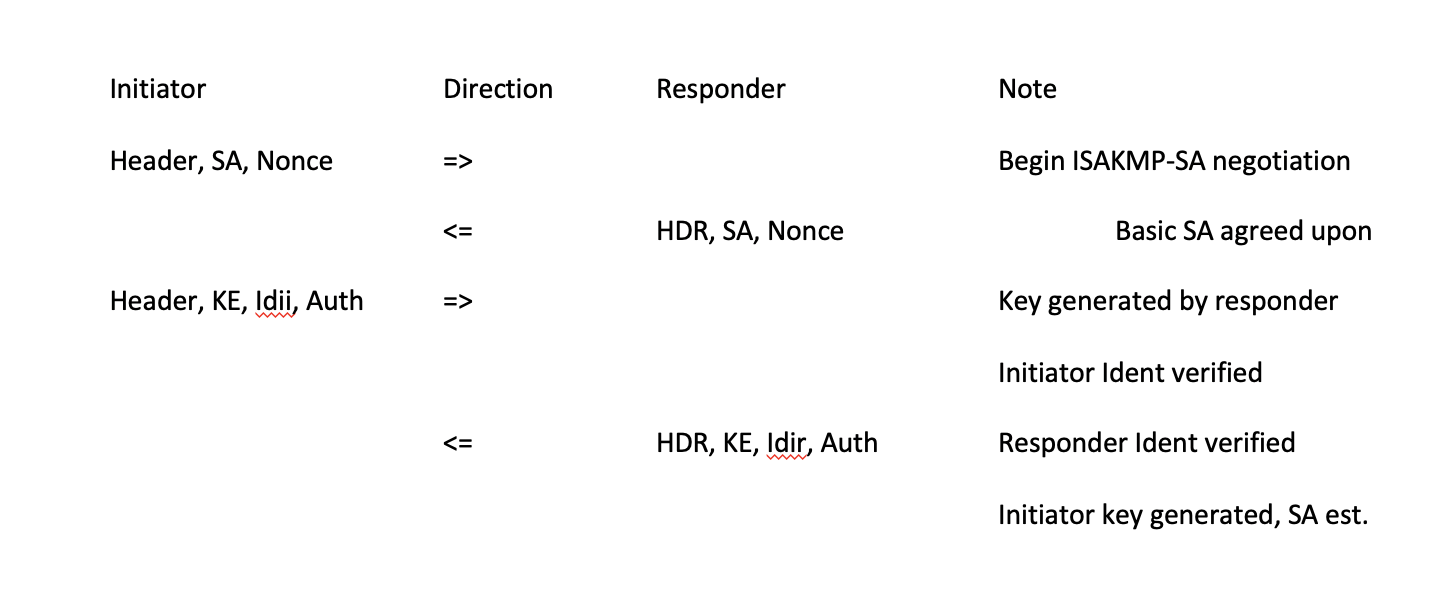
\includegraphics[width=\textwidth] {ISAKMP_Neg_Procedure}

Another example details the IKE procedures which is two phases. Phase one establishes a secure channel and phase two transmitts data. Below is an example  with more detail in regards to the two phases.

For phase 1:
\begin{enumerate}
\item Initator sends proposed policies
\item Responder will accept one and reply
\item Initiator generates DH (Diffie Hellman outlined in IKE) and sends them
\item Responder generates DH values
  \begin{itemize}
  \item Both ends now use the DH values to generate a DH shared secret
  \end{itemize}
\item Initiator sends its ID and hash of preshared key for authentication
\item Responder sends its ID and hash of preshared key. Both ends check if hashes match.
\end{enumerate}

Phase 1 final outcome: tunnel for negotiation of further security parameters

For phase 2:
\begin{enumerate}
  \item Initiator sends additional parameters to responder
    \begin{itemize}
      \squash
    \item encapsulation method
    \item hashing method
    \item DH group
    \item SPI
    \end{itemize}
  \item Responder accepts proposal and sends its own SPI and matching parameters
    \begin{itemize}
    \item Bothends generate new DH keys for encryption
    \end{itemize}
  \item The initiator acknowledges the message was recieved. This establishes the Security Association.
\end{enumerate}

Phase 2 final outcome: any traffic passing over the tunnel is now encrypted and will continue to be until the tunnel is terminated. Also, a SA between the two endpoints is established using Phase 1's tunnel. This is in turn a security context. 

\chapter {Works Cited}

\begin{enumerate}
\item https://www.computerweekly.com/news/2240102144/What-is-the-ISAKMP-policy-and-how-does-it-impact-IPsec-VPN-router-configuration
\item 8.2.5.IPSec-ISAKMP.ppt
\item https://networkdirection.net/articles/network-theory/ipsecbasics/
\item https://training.apnic.net/wp-content/uploads/sites/2/2016/11/eSEC03_IPSec_Basics.pdf
\end{enumerate}
 

\end{document}
